\documentclass[twocolumn,linenumbers]{aastex701}

\journalinfo{}
\makeatletter
\renewcommand{\frontmatter@title@above}{}
\makeatother
\AtBeginDocument{\hypersetup{colorlinks=true,linkcolor=black,citecolor=black,urlcolor=xlinkcolor,filecolor=black}}
\shorttitle{}
\shortauthors{}
 

% Local production preview style: suppress running heads and place page numbers
% at the bottom center. AAS production will apply the final published style.
\makeatletter
\def\ps@apjheads{%
  \let\@mkboth\@gobbletwo
  \let\@oddhead\@empty
  \let\@evenhead\@empty
  \def\@oddfoot{\hfil\thepage\hfil}%
  \def\@evenfoot{\hfil\thepage\hfil}%
}
\def\ps@plain{%
  \let\@mkboth\@gobbletwo
  \let\@oddhead\@empty
  \let\@evenhead\@empty
  \def\@oddfoot{\hfil\thepage\hfil}%
  \def\@evenfoot{\hfil\thepage\hfil}%
}
\def\ps@titlepage{%
  \let\@mkboth\@gobbletwo
  \let\@oddhead\@empty
  \let\@evenhead\@empty
  \def\@oddfoot{\hfil\thepage\hfil}%
  \def\@evenfoot{\hfil\thepage\hfil}%
}
\makeatother
\pagestyle{plain}

\begin{document}
\pagestyle{plain}

 \title{Supplementary Material for "A Geometric-Medium Response Phenomenology for SPARC Rotation Curves"}
 \author{Mohammed Messaoudene}
\altaffiliation{Corresponding author: Mohammed Messaoudene; email: \href{mailto:mohammed.messaoudene@univ-temouchent.edu.dz}{mohammed.messaoudene@univ-temouchent.edu.dz}; ORCID iD: \href{https://orcid.org/0009-0007-4665-2548}{0009-0007-4665-2548}.}
 \affiliation{Faculty of Sciences, Belhadj Bouchaib University of Ain Temouchent, Route of Sidi Bel Abbes, BP 284, 46000 Ain Temouchent, Algeria}
 \email{mohammed.messaoudene@univ-temouchent.edu.dz}

\section{Appendix A. Data ingestion and sample accounting}

Throughout the analysis we use the Geometric-Medium Response (GMR) model as the editorial name. Implementation identifiers are excluded from the public prose and retained only in provenance tables where artifact traceability requires them.

This supplement documents the archived analysis products associated with the manuscript. It does not rerun the entire upstream SPARC ingestion workflow from public source archives. Instead, it records the finalized machine-readable tables, figure-source CSVs, and derived summaries that support the paper. The authoritative sample table contains 175 galaxies and confirms that the figure rule excluding galaxies with fewer than eight observed points from the main rotation-curve atlas is preserved.



\begin{deluxetable}{ll}
\tablecaption{Sample accounting carried into the fixed study.}
\tablehead{\colhead{Quantity} & \colhead{Value}}
\startdata
Full SPARC sample galaxies & 175 \\
Held-out fixed subset galaxies & 151 \\
Mass-model rows & 3391 \\
Galaxies with $N_{\rm obs}<5$ & 4 \\
Galaxies with $N_{\rm obs}<8$ & 32 \\
Main-text visual rule & Exclude galaxies with $N_{\rm obs}<8$ \\
\enddata
\end{deluxetable}

The accounting matters because a galaxy with three observed points and a galaxy with thirty observed points both count once in the equal-weight aggregate, yet they should not occupy the same rhetorical space in a main-text figure discussion. The supplement therefore preserves the low-information flags and the main-panel threshold explicitly.
\section{Appendix B. Metric definitions}

Equal-weight RMSE is defined by treating each galaxy-level RMSE as one sample and then taking the root-mean-square across galaxies. Mean absolute residual and the headline median absolute residual are carried directly from the archived aggregate metrics table when available. The headline median values are pooled absolute-residual medians from that aggregate table; medians recomputed over galaxy-level median columns give 16.167 km s$^{-1}$ for GMR and 8.401 km s$^{-1}$ for reduced NFW on the full sample and are treated only as a robustness check. Per-galaxy win rate is the fraction of galaxies for which the GMR residual metric is smaller than the comparator's residual metric.

The model comparisons are treated as descriptive performance diagnostics rather than as family-wise significant inferential claims. Under a joint Holm-Bonferroni correction across the four RMSE contrasts, no contrast remains below $\alpha=0.05$. The held-out 151-galaxy equal-weight-RMSE comparison is reported as the main descriptive aggregate metric. Mean, median, win rate, RAR, BTFR, and the class-level stress tests remain essential, but they function as descriptive diagnostic quantities rather than as a second layer of confirmatory hypothesis tests.

The supplement also standardizes one bootstrap wording rule: \texttt{bootstrap\_negative\_fraction} means the fraction of bootstrap replicates with $\Delta$RMSE $< 0$. It is not a posterior probability and should not be described that way in the manuscript or cover letter.



\section{Appendix C. Rotation-curve atlas details and figure-source provenance}

The extended rotation-curve atlas is provided in the public repository; the main text shows representative examples only.

The figure manifest ties each panel to a real source CSV and the final polished PNG assets. Main-text Figure 1 contains six panels: bulge success (UGC02487), bulge tension (NGC5371), ordinary-disk success (UGC02885), ordinary-disk tension (UGC06930), dwarf success (UGC00128), and dwarf tension (UGC07125). The extended atlas retains NGC3741, UGC05918, UGC07323, and UGC11914 for context.

\begin{figure*}[t]
\centering
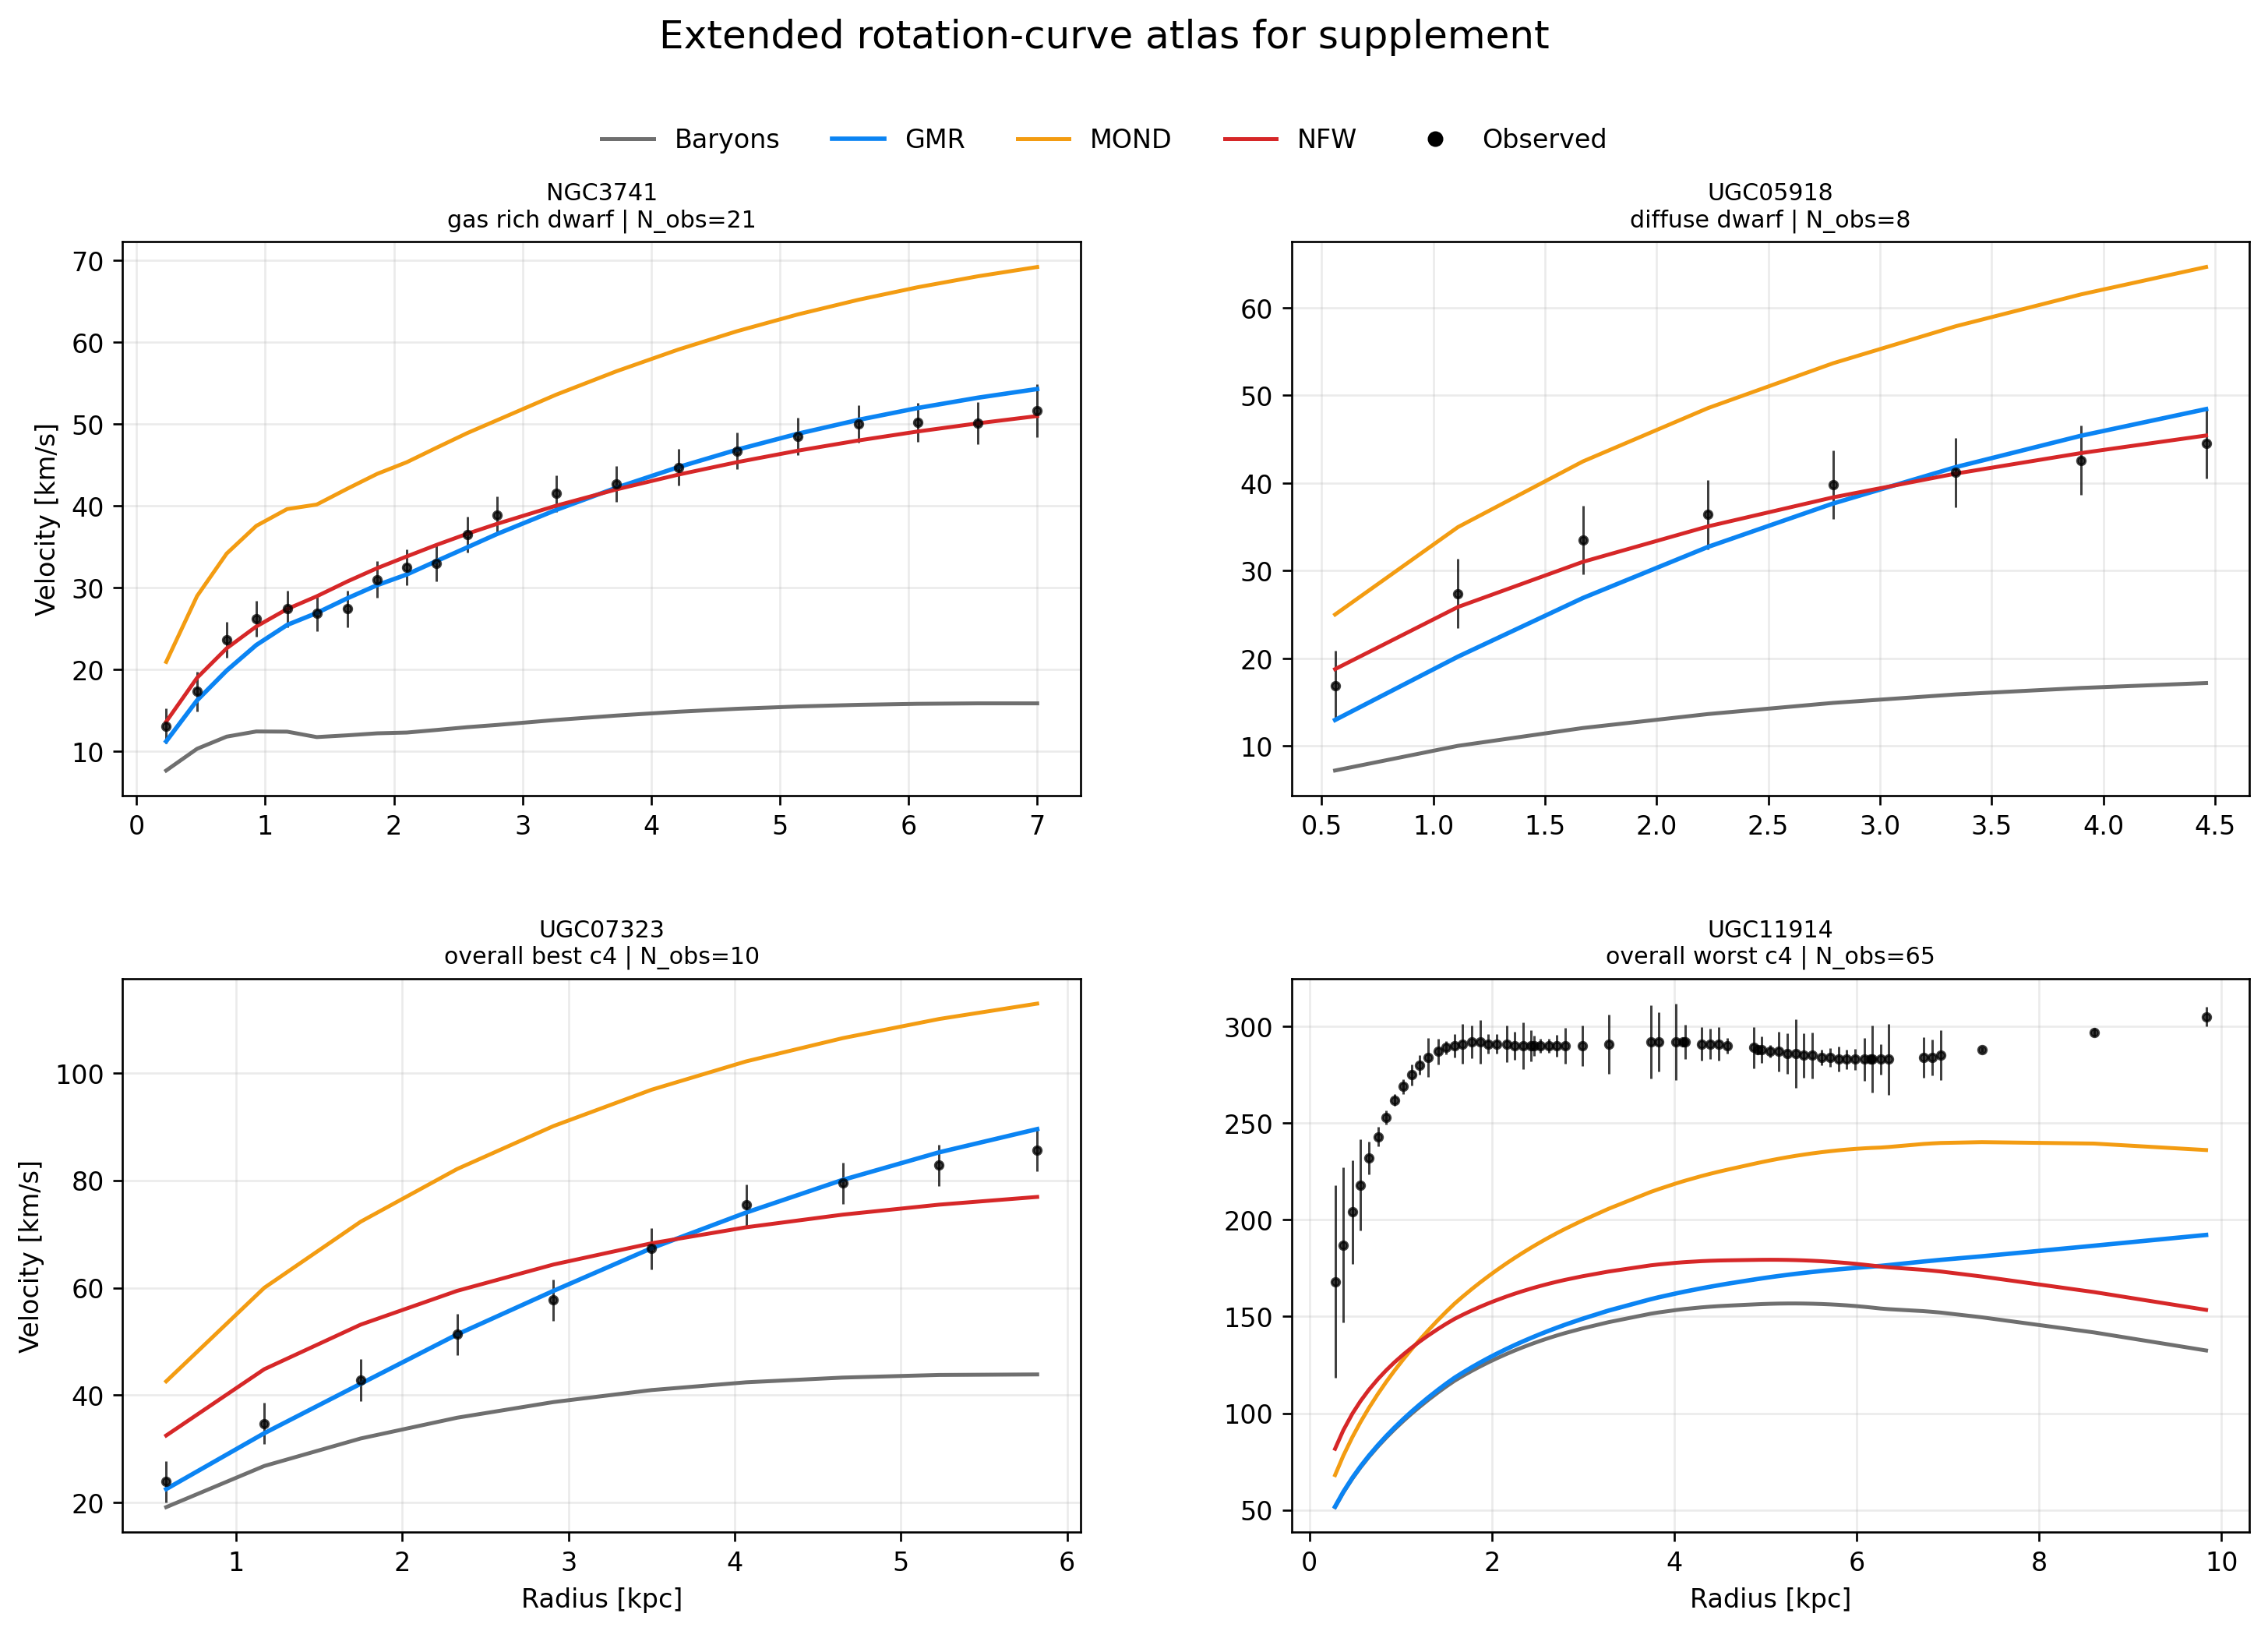
\includegraphics[width=\textwidth]{figures/FIGS1_extended_rotation_atlas.png}
\caption{Extended rotation-curve atlas carrying the additional context panels used during the figure-polish phase. These panels remain in the analysis for transparency but are not all promoted to the main text.}
\end{figure*}

The corresponding figure-source CSVs are listed in the figure manifest so that a reader can connect the rendered PNGs back to machine-readable panel inputs.

Panel selection followed two rules that are easy to forget if they are not written down. First, the main-text atlas had to satisfy the minimum-information rule $N_{\rm obs}\ge 8$. Second, the final panel set had to balance success and tension cases across the morphology slices rather than selecting only the most flattering visuals. These rules explain why certain attractive but low-information galaxies appear only in the supplement and why some visibly tense panels remain in the main text.

Provenance is preserved at two layers. The copied final figure manifest records the intended semantic role of each panel and the immediate source CSVs. The \texttt{source\_csv} directory then stores those CSVs inside the submission artifact set. This keeps the figure provenance auditable without turning the supplement into an implementation log.

The extended atlas is not decorative. It gives the reader access to diffuse dwarf, gas-rich dwarf, and extreme best/worst examples that would otherwise be only summarized verbally. Keeping those panels in the supplement allows the main paper to stay readable without sacrificing transparency.
\section{Appendix D. RAR calculation details}

The final RAR table contains both full-sample point rows and full-sample binned rows. The binned rows carry residual columns named \texttt{c4\_minus\_official} and \texttt{mond\_minus\_official}. Recomputing the root-mean-square of those stored binned residuals yields 0.0640 for GMR and 0.2032 for MOND. The archived RAR products use 13 equal-weight stored binned residual rows for the GMR and MOND binned series over log $g$ range -11.69 to -9.12; official comparison bins are stored separately in \texttt{rar\_binning\_spec.csv}.

This result is interpreted as a within-sample consistency diagnostic rather than as an independent validation set. The fixed global amplitude was selected on a SPARC calibration subset, so the RAR is informative but not external. The paper therefore uses the RAR to support internal coherence of the fixed implementation, not to replace the rotation-curve caveats.



\section{Appendix E. BTFR calculation details}

The BTFR table carries per-galaxy rows and fit-summary rows. The fit summaries show 123 galaxies contributing to the observed $V_{\rm flat}$ fit and the same number contributing to the fixed GMR proxy fit. The present paper cites the fit-summary rows directly rather than reconstructing the fit from scratch, because those rows are already the machine-readable fixed product authorized for the fixed study.

The smaller galaxy count relative to the full SPARC benchmark is not an inconsistency. The BTFR fit is defined only for galaxies with a usable flat-velocity observable in the fixed table. Several per-galaxy rows contain zero or unavailable velocity values, which means they legitimately drop out of the fit-summary stage. The manuscript keeps this distinction visible so that the BTFR section cannot be misread as a 175-galaxy fit.

As in the main text, the supplement separates slope and scatter. The slope agreement is good enough for a supportive statement, but the larger scatter is the reason the BTFR remains secondary evidence rather than a headline claim. Preserving that internal balance is one of the goals of the analysis.
\section{Appendix F. Bootstrap and jackknife procedures}

Bootstrap diagnostics are checked directly from the archived per-galaxy metrics file with a fixed random seed (20260421). Percentile intervals use 10000 paired resamples, while the canonical BCa summary table records 5000 paired resamples. The canonical outputs are stored in the repository's FIG5 bootstrap source CSV and used wherever exact bootstrap numbers are quoted.

\begin{deluxetable*}{lrrrrr}
\tabletypesize{\scriptsize}
\tablecaption{Canonical bootstrap and jackknife outputs used in the final fixed analysis.}
\tablehead{\colhead{Subset} & \colhead{Comparator} & \colhead{$\Delta$ RMSE} & \colhead{Percentile 95\% CI} & \colhead{BCa 95\% CI} & \colhead{Bootstrap-negative fraction}}
\startdata
full\_175 & MOND & -4.353 & [-8.959, 0.228] & [-8.783, 0.660] & 0.969 \\
full\_175 & NFW & -6.059 & [-11.444, -0.728] & [-12.147, -1.243] & 0.987 \\
heldout\_151 & MOND & -3.497 & [-8.721, 1.531] & [-8.453, 1.701] & 0.910 \\
heldout\_151 & NFW & -6.580 & [-12.538, -0.550] & [-13.089, -1.038] & 0.985 \\
\enddata
\end{deluxetable*}

The outlier-influence table remains important because it answers a different question. Single-galaxy jackknife never flips the sign, but a small set of highly favorable galaxies can. On the held-out subset, the archived outlier table shows sign reversal after removing 9 highly favorable galaxies against MOND and 9 against reduced NFW. These results show that sign reversal requires removal of a small set of highly favorable galaxies rather than a single object.



\section{Appendix G. Dwarf and low-surface-brightness failure modes}

The class-level and correlation diagnostics support a consistent failure-mode picture. Gas fraction correlates positively with GMR-minus-NFW failure (0.270), while effective surface brightness and total luminosity correlate negatively. The low-mass-dwarf class is the clearest systematic weakness, with a GMR-versus-reduced-NFW win rate of only 0.136. The top-failure list nonetheless includes both dwarfs and bulge-rich outliers, so the analysis explicitly says "principal tension" rather than "exclusive tension."

Top-failure summary: NGC5371 (bulge-rich HSB, GMR minus NFW 79.292); NGC0801 (bulge-rich HSB, GMR minus NFW 69.282); F574-2 (low-mass dwarf, GMR minus NFW 35.595); UGC07125 (low-mass dwarf, GMR minus NFW 34.273); UGC06628 (low-mass dwarf, GMR minus NFW 31.975); UGC09037 (bulge-rich HSB, GMR minus NFW 29.947). Correlation summary: \texttt{sbeff\_sol\_lum\_pc2} = -0.164, \texttt{gas\_fraction\_proxy} = 0.270, \texttt{luminosity\_36e9\_sol} = -0.463, \texttt{rdisk\_kpc} = -0.252, \texttt{reff\_kpc} = -0.414.

The distinction between class-average weakness and extreme individual outliers is central. Class-average metrics show where the fixed prescription underperforms. The top-failure table shows where the single-galaxy misses are largest. Those two views overlap, but they are not identical. The supplement keeps both because together they explain why low-density regimes matter while also preventing an overly tidy narrative.

Leave-class-out tests sharpen that point. Removing low-mass dwarfs does not erase the reduced-NFW comparison; removing bulge-rich high-surface-brightness galaxies does. The aggregate leverage therefore comes heavily from the bulge-rich class even though the systematic weakness lives in the low-density classes. This tension between leverage and weakness is one of the most informative scientific outputs of the analysis.

For future theory work, that pattern suggests where added structure would have to enter. For the fixed study, however, it serves a different role: it tells the referee exactly where the current fixed response closure is strongest and where it remains incomplete.
\section{Appendix H. Out-of-scope local and screening claims}

This appendix exists only to prevent scope confusion. The phenomenological suppression factor inside the fixed galaxy equations is part of the public GMR model, but this paper does \textbf{not} treat that term as a proof of local screening or as a tested local-gravity closure. No PPN, Cassini, binary-pulsar, laboratory, or gravitational-wave-speed claim is made here.

In other words, local screening is not established in this work and is not used as a central claim.
\section{Appendix I. Out-of-scope cosmology and backend claims}

Earlier analysis products stages explored backend and cosmological witness layers, but they are not part of the evidential claim of the present paper. This article does not rely on CLASS readiness, Einstein-Boltzmann closure, cluster phenomenology, strong-field behavior, or dark-energy closure. Those sectors are outside the scope of this article.
\section{Appendix J. Scope summary}

The scope summary is intentionally narrow. The reported results are: aggregate equal-weight-RMSE improvement over baryons, MOND, and reduced NFW; stronger reduced ISO/Burkert aggregate performance overall; strong within-sample RAR consistency; supportive but imperfect BTFR consistency; and explicit dwarf/LSB limitations. No screening, cosmology, cluster, or strong-field success claim appears in this work.



 \section{Appendix K. Stratified robustness summary}

The fixed stress table exports three preregistered morphology slices: bulge-rich high-surface-brightness systems, low-mass dwarfs, and ordinary disks. Those are the stratified comparisons that can be reproduced directly from the archived tables without inventing new class boundaries at submission time.

\begin{deluxetable}{lrrrrrr}
\tablecaption{Stratified metrics available from the fixed stress table.}
\tablehead{\colhead{Slice} & \colhead{N} & \colhead{GMR} & \colhead{MOND} & \colhead{NFW} & \colhead{ISO} & \colhead{GMR/NFW WR}}
\startdata
bulge-rich HSB & 77 & 58.080 & 59.306 & 68.390 & 29.602 & 0.532 \\
low-mass dwarf & 81 & 15.523 & 27.778 & 6.880 & 4.478 & 0.136 \\
ordinary disk & 17 & 22.428 & 33.944 & 30.933 & 13.576 & 0.235 \\
\enddata
\end{deluxetable}

\section{Appendix L. Per-galaxy GMR versus reduced-NFW differences}

The per-galaxy delta histogram provides a complementary view of the same comparison. Although GMR remains ahead of reduced NFW on aggregate equal-weight RMSE, the galaxy-by-galaxy distribution is asymmetric in the opposite direction.

\begin{figure*}[t]
\centering
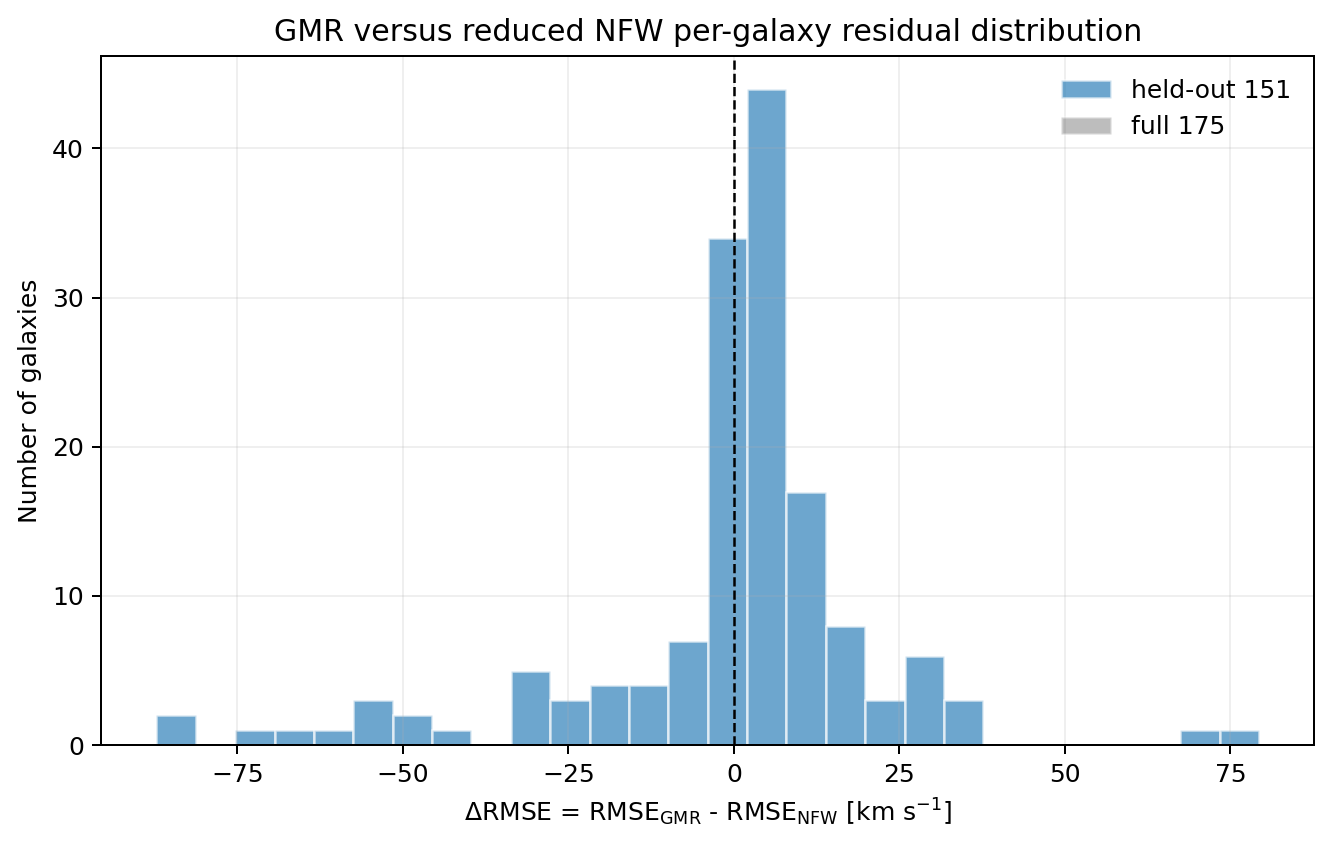
\includegraphics[width=\textwidth]{figures/FIG7_GMR_vs_NFW_delta_histogram.png}
\caption{Per-galaxy delta RMSE = RMSE$_{\rm GMR}$ - RMSE$_{\rm NFW}$ for the full and held-out samples. Negative values favor GMR.}
\end{figure*}

\begin{figure*}[t]
\centering
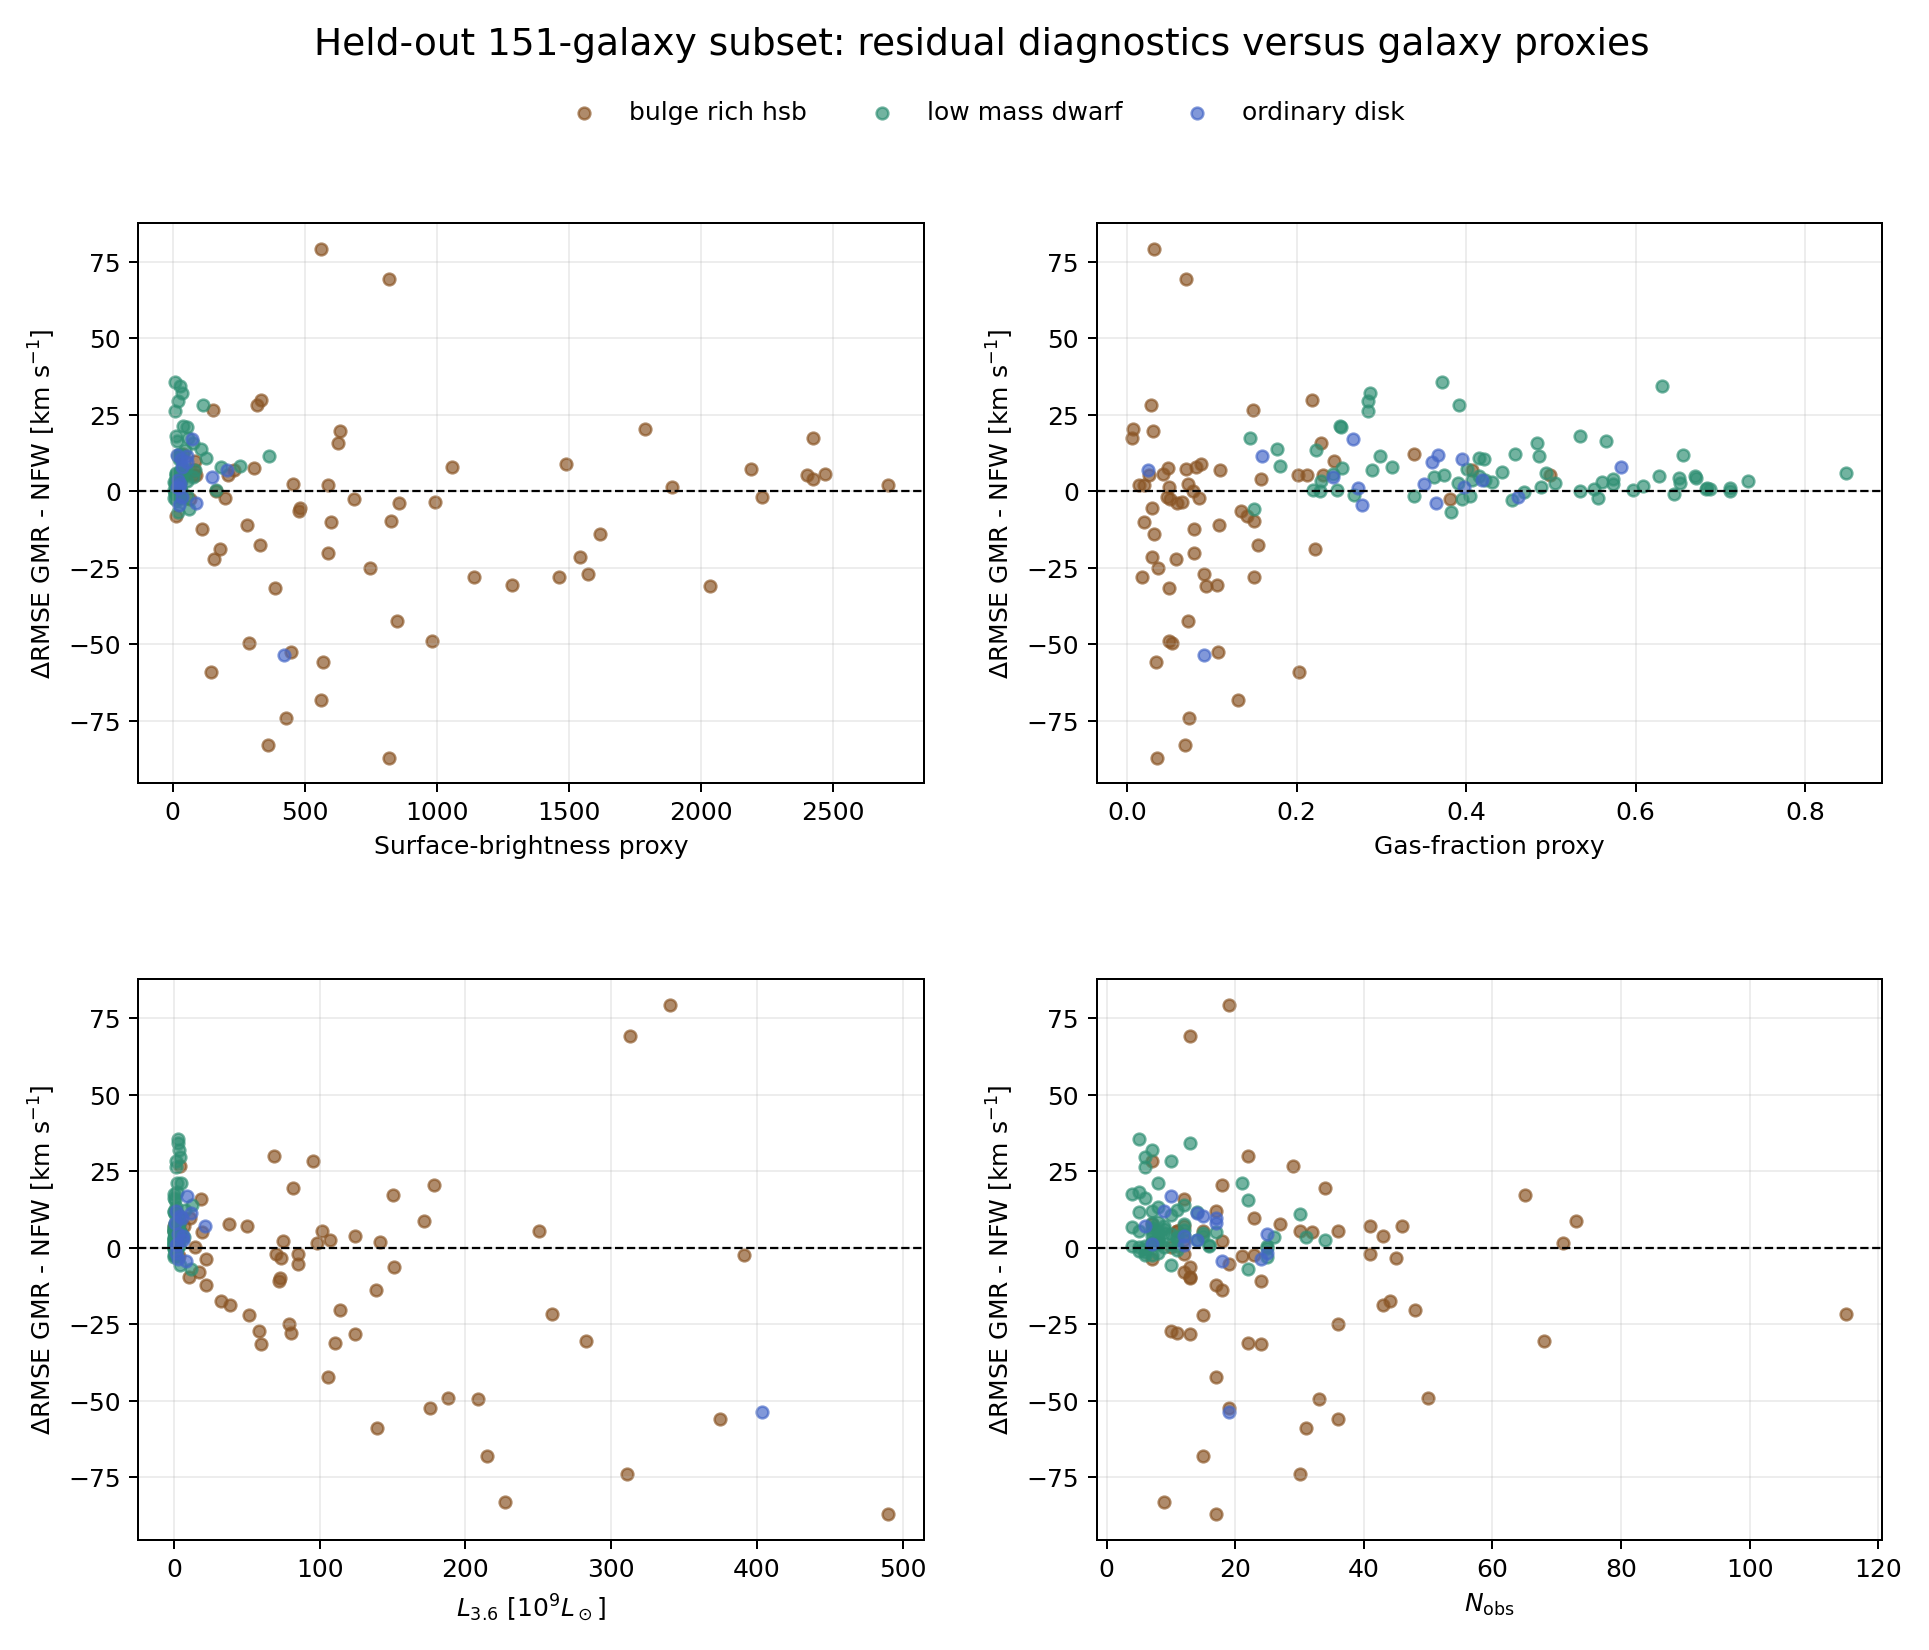
\includegraphics[width=\textwidth]{figures/FIG6_residuals_vs_properties.png}
\caption{Per-galaxy delta RMSE (GMR - NFW) on the held-out subset as a function of surface-brightness, gas-fraction, luminosity, and sampling proxies.}
\end{figure*}

\section{Appendix M. Outlier leverage and sign-reversal thresholds}

Jackknife alone does not reverse the aggregate sign against MOND or reduced NFW on the fixed benchmark, but a small set of highly favorable galaxies can. The full-sample sign-reversal thresholds are 12 removals for MOND and 9 for reduced NFW, while the held-out-subset thresholds are 9 and 9.

\begin{figure*}[t]
\centering
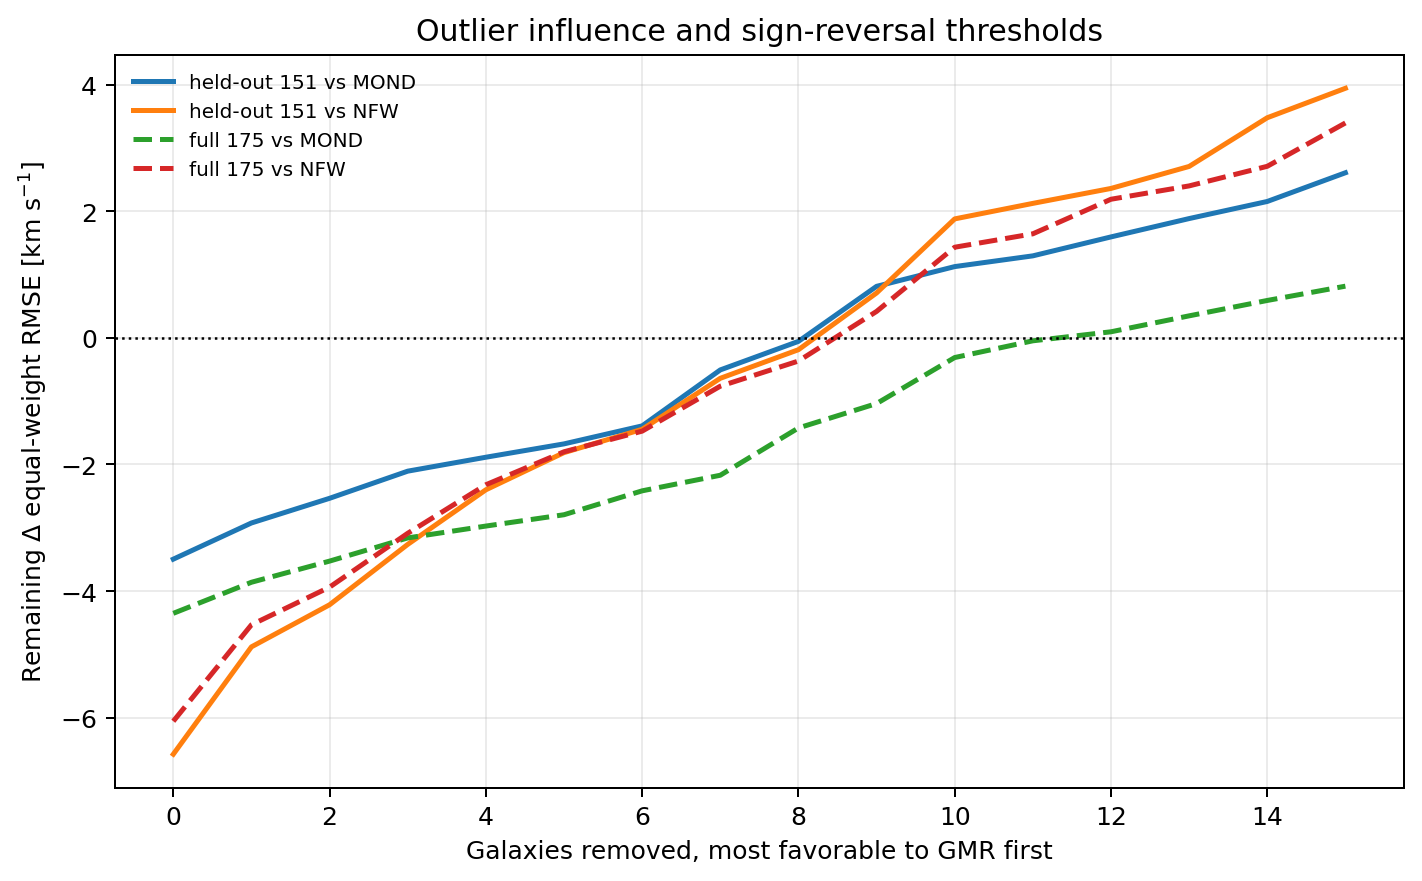
\includegraphics[width=\textwidth]{figures/FIG8_outlier_influence.png}
\caption{Change in aggregate delta equal-weight RMSE as the most favorable GMR galaxies are removed from the sample.}
\end{figure*}

\section{Appendix N. Extended atlas provenance}

The extended rotation atlas remains in the supplement because it is the cleanest way to show context galaxies without overloading the main text. Every panel keeps its source CSV, and panels with low N$_{\rm obs}$ remain supplementary context rather than primary proof.
\section{Appendix O. Equation provenance and fixed parameter table}

The displayed GMR equations in the main manuscript are not editorial inventions. They are transcribed from the stored implementation that generated the paper-level tables and figures. The public repository release stores the provenance scripts under \texttt{scripts/provenance/}, the fixed parameter record under \texttt{docs/provenance/}, and the final paper-level tables plus figure-source CSVs under \texttt{tables/} and \texttt{source\_csv/}. The public provenance table in the repository maps those files to the equations and diagnostics used in this paper.

The public provenance table, fixed parameter record, and parameter inventory are the authoritative archived sources for traceability. They also record the public rounding convention for the response amplitude: the manuscript uses $\mathcal{A}_{\rm GMR} \approx 1.395\times10^{-5}$ in prose, while the exact fixed machine value $1.3945832491957465\times10^{-5}$ is preserved in the reproducibility table only.



\section{Final clarifications on archived stress-test bins and comparator use}
The final analysis treats the morphology and surface-brightness labels used in the
stress-test tables as archived diagnostic bins rather than newly inferred
physical classifications. The final machine-readable class counts are
$77/81/17$ across the archived bins used for the paper-level summaries. The manuscript and supplement use these archived diagnostic bins consistently for the reported class-level stress tests.

The reduced halo comparisons in the paper are likewise treated as archived
baselines. They are retained to expose the local flexibility advantage of
per-galaxy halo descriptions, not to claim equal parameter accounting with the
fixed GMR response. The manuscript therefore compares the archived
observable residual columns and keeps the parameter-freedom asymmetry explicit.



\section{Appendix P. Provenance label mapping}

For reproducibility, some archived files retain their historical internal filenames. Public prose uses neutral provenance labels. The mapping is:

\begin{deluxetable*}{ll}
\tablecaption{Public provenance labels used in this supplement.}
\tablehead{\colhead{Public label} & \colhead{Reproducibility role}}
\startdata
\texttt{gmr\_stage\_c2\_validation.py} & baryonic source record and Newtonian acceleration import \\
\texttt{gmr\_stage\_c4\_2\_response\_validation.py} & baryonic invariant construction and regularization constants \\
\texttt{gmr\_statevar\_symbolic\_regression.py} & cumulative state proxy and closure form \\
\texttt{gmr\_fixed\_parameter\_record.md} & fixed response-parameter record used for reproducibility \\
\enddata
\end{deluxetable*}


\section{Appendix Q. Supplementary method-sensitivity audit}

This appendix records the method-hardening consequences of the final hostile-review pass. The main manuscript remains a SPARC galaxy-phenomenology paper and no GMR prediction is retuned here. The new supplementary method-sensitivity tables add multi-metric sensitivity, tail decomposition, conservative parameter-count diagnostics, calibration-subset provenance, dimensional checks, and observational-systematics disclosure.

The main interpretive changes are: (1) the equal-weight RMSE result is treated as an aggregate tail-robustness result, not typical-galaxy superiority; (2) the 151-galaxy comparison set is described as held-out relative to the final two-parameter calibration, not as an independently preregistered data set; (3) fixed structural constants are counted as effective model complexity in conservative diagnostics; (4) no matched global-halo baseline is claimed to have been implemented; and (5) the method-sensitivity artifacts listed in the repository release are included as files with the \texttt{method\_} prefix for exact traceability.

The machine-readable method-sensitivity files are included with the package using the \texttt{method\_} prefix; the exact filenames are enumerated in the repository manifest and in \texttt{METHOD\_FILES.md}.

\section{Appendix R. Reproducibility limitations}

The public release is designed to reproduce the reported aggregate metrics, bootstrap tables, figure-source products, parameter records, and manuscript figures from the archived derived tables. It does not claim to regenerate the full SPARC mass-model pipeline from raw photometry, distance choices, inclination choices, or stellar mass-to-light assumptions. The SPARC input data remain publicly available from the SPARC database, while this release provides the derived per-galaxy table, figure-source CSVs, metric recomputation script, repository-integrity checker, and LaTeX source used for the paper.

This distinction is important for interpretation. The repository supports verification of the reported tables and figures, but it is not a full raw-SPARC refitting environment and does not propagate distance, inclination, or stellar mass-to-light uncertainties. The corresponding limitation is stated in the main text by treating the comparisons as descriptive performance diagnostics rather than as complete uncertainty-propagated model selection.

\section{Appendix S. Calibration subset provenance}

The 24 calibration galaxies are archived explicitly in the release. This subset is used only to document the final two-parameter calibration provenance; the 151-galaxy comparison set is held out relative to that final calibration, not an independently preregistered external sample.

\begin{deluxetable*}{llllll}
\tabletypesize{\scriptsize}
\tablecaption{Calibration\_24 subset provenance. Surface brightness and gas-fraction proxies are the archived columns carried in the canonical per-galaxy metrics table.}
\tablehead{\colhead{Galaxy} & \colhead{Class} & \colhead{$\Sigma_{\rm eff}$ proxy} & \colhead{Gas fraction proxy} & \colhead{$N_{\rm obs}$} & \colhead{Role}}
\startdata
CamB & low\_mass\_dwarf & 7.89 & 0.138 & 9 & calibration \\
D512-2 & low\_mass\_dwarf & 9.22 & 0.200 & 4 & calibration \\
DDO154 & low\_mass\_dwarf & 20 & 0.838 & 12 & calibration \\
DDO161 & low\_mass\_dwarf & 20.7 & 0.715 & 31 & calibration \\
DDO170 & low\_mass\_dwarf & 9.39 & 0.575 & 8 & calibration \\
IC4202 & bulge\_rich\_hsb & 392 & 0.064 & 32 & calibration \\
KK98-251 & low\_mass\_dwarf & 7.89 & 0.575 & 15 & calibration \\
NGC0247 & ordinary\_disk & 33.8 & 0.192 & 26 & calibration \\
NGC0289 & bulge\_rich\_hsb & 1.59e+03 & 0.276 & 28 & calibration \\
NGC1003 & bulge\_rich\_hsb & 141 & 0.463 & 36 & calibration \\
NGC1705 & low\_mass\_dwarf & 347 & 0.207 & 14 & calibration \\
NGC2403 & bulge\_rich\_hsb & 341 & 0.242 & 73 & calibration \\
NGC2915 & low\_mass\_dwarf & 347 & 0.442 & 30 & calibration \\
NGC2955 & bulge\_rich\_hsb & 975 & 0.083 & 24 & calibration \\
NGC3741 & low\_mass\_dwarf & 42.9 & 0.867 & 21 & calibration \\
NGC4138 & bulge\_rich\_hsb & 1.91e+03 & 0.033 & 7 & calibration \\
NGC5055 & bulge\_rich\_hsb & 1.38e+03 & 0.071 & 28 & calibration \\
NGC6503 & bulge\_rich\_hsb & 774 & 0.120 & 31 & calibration \\
NGC6946 & bulge\_rich\_hsb & 571 & 0.079 & 58 & calibration \\
UGC03580 & bulge\_rich\_hsb & 615 & 0.248 & 47 & calibration \\
UGC05721 & bulge\_rich\_hsb & 234 & 0.514 & 23 & calibration \\
UGC05764 & low\_mass\_dwarf & 9.31 & 0.657 & 10 & calibration \\
UGC06973 & bulge\_rich\_hsb & 3.32e+03 & 0.032 & 9 & calibration \\
UGCA444 & low\_mass\_dwarf & 11.9 & 0.848 & 36 & calibration \\
\enddata
\end{deluxetable*}



\section{Appendix T. Recovered radial diagnostics included in the public release}

The release includes all-galaxy radial invariant and prediction tables, the 3391-point $\sin\alpha_B S_{\rm rad}$ diagnostic, a pure $\sqrt{g_N}$ baseline optimized on \texttt{calibration\_24}, and a local-$S_\Psi=\nu_B/(1+\nu_B)$ variant. The archived release is available at \url{https://doi.org/10.5281/zenodo.20032301}, with development source at \url{https://github.com/mohammedmessaoudene-cmd/GMR-SPARC-Paper1}.

\begin{deluxetable}{lrrrr}
\tablecaption{Recovered square-root and local-state diagnostics. RMSE values are equal-weight per-galaxy aggregates in km\,s$^{-1}$.}
\tablehead{\colhead{Model} & \colhead{Full} & \colhead{Calibration} & \colhead{External} & \colhead{Nobs full}}
\startdata
GMR recovered & 40.554 & 31.021 & 41.870 & 57.334 \\
MOND recovered & 44.907 & 41.903 & 45.366 & 52.224 \\
Pure $\sqrt{g_N}$ baseline & 40.241 & 32.579 & 41.329 & 54.835 \\
GMR local-$S_\Psi$ variant & 47.683 & 35.019 & 49.398 & 66.504 \\
\enddata
\end{deluxetable}

The fitted pure-square-root amplitude is $9.0294884547\times10^{-6}$, optimized on \texttt{calibration\_24} with a bounded scalar search over the same amplitude interval spanned by the archived amplitude grid. The diagnostic factor $\sin\alpha_B S_{\rm rad}$ is not constant: across the 3391 recovered points its median is 0.599, with a 5--95 percentile range of 0.063--0.967. The local-$S_\Psi$ replacement gives equal-weight RMSE 47.683 km\,s$^{-1}$ on the full sample and 49.398 km\,s$^{-1}$ on the held-out subset, so the cumulative state variable improves over this tested local replacement. The pure square-root baseline slightly outperforms GMR on the equal-weight aggregate, so the supplement treats this as a constraint on the tested geometric-invariant architecture rather than a secondary caveat. This is treated as a limitation on GMR distinctiveness rather than as a failure of the reproduced GMR metrics.

\end{document}
